

\documentclass[a4paper,12pt]{report}

% --- 0 nome appunti


% --- 1. LINGUA E FONT ---
\usepackage[T1]{fontenc}
\usepackage[utf8]{inputenc}
\usepackage[italian]{babel} % Traduce "Chapter" in "Capitolo", ecc.
\usepackage{lmodern}        % Font vettoriale di alta qualità
\usepackage{ulem}
\usepackage{multirow}
\usepackage{makecell}

% --- 2. GEOMETRIA E IMPAGINAZIONE ---
\usepackage[a4paper, top=2.5cm, bottom=2.5cm, left=2.5cm, right=2.5cm]{geometry}
\usepackage{titlesec}       % Personalizzazione dei titoli
\setlength{\parindent}{0pt}
% Rimuove la scritta "Capitolo X" e affianca il numero al titolo
\titleformat{\chapter}[hang]
  {\normalfont\huge\bfseries}{\thechapter.}{20pt}{\Huge}
\titlespacing*{\chapter}{0pt}{-20pt}{30pt}

% --- 3. MATEMATICA E SIMBOLI ---
\usepackage{amsmath, amssymb, amsfonts}

% --- 4. GRAFICA E IMMAGINI ---
\usepackage{graphicx}
\usepackage{float}          % Permette l'uso di [H] per forzare la posizione delle immagini
\usepackage{caption}        % Personalizzazione delle didascalie
\usepackage{subcaption}     % Per affiancare più immagini
\usepackage{geometry}
\geometry{a4paper, margin=1.25cm}
\usepackage{parskip}
\usepackage{titlesec}
\usepackage{xltabular}

% --- 5. TIKZ ---
\usepackage{tikz}

% --- 6. LISTE E TABELLE ---
\usepackage{enumitem}       % Controllo avanzato di itemize e enumerate
\usepackage{booktabs}       % Tabelle professionali (toprule, midrule, bottomrule)
\usepackage{tabularx}       % Tabelle che si adattano alla larghezza della pagina

% --- 7. FORMATTAZIONE DEL CODICE (LISTINGS) ---
\usepackage{listings}
\usepackage{xcolor}

% Definizione colori per il codice
\definecolor{codegreen}{rgb}{0,0.6,0}
\definecolor{codegray}{rgb}{0.5,0.5,0.5}
\definecolor{codepurple}{rgb}{0.58,0,0.82}
\definecolor{backcolour}{rgb}{0.95,0.95,0.92}

% Configurazione stile codice (ottimizzato per Java/C++)
\lstdefinestyle{oopstyle}{
    backgroundcolor=\color{backcolour},   
    commentstyle=\color{codegreen}\itshape,
    keywordstyle=\color{magenta}\bfseries,
    numberstyle=\tiny\color{codegray},
    stringstyle=\color{codepurple},
    basicstyle=\ttfamily\footnotesize,
    breakatwhitespace=false,         
    breaklines=true,                 
    captionpos=b,                    
    keepspaces=true,                 
    numbers=left,                    
    numbersep=5pt,                  
    showspaces=false,                
    showstringspaces=false,
    showtabs=false,                  
    tabsize=2,
    frame=single,
    rulecolor=\color{black!30}
}
\lstset{style=oopstyle}

% --- 8. BOX COLORATI (PATTERN GRASP, GOF, PROCESSO UP) ---
\usepackage[most]{tcolorbox}

% --- 9. COLLEGAMENTI E INDICE (Da caricare per ultimo) ---
\usepackage{hyperref}
\hypersetup{
    colorlinks=true,
    linkcolor=blue!70!black, % Colore dei link interni (indice)
    filecolor=magenta,       % Colore dei link a file
    urlcolor=cyan,           % Colore degli URL
    pdftitle={Appunti di Architettura degli elaborati},
    pdfauthor={Il tuo nome},
    pdfpagemode=UseOutlines
}
\usepackage{bookmark} % Migliora i segnalibri nel lettore PDF

\begin{document}

    \begin{titlepage}
        \centering
        
        \begin{center}
            
\includegraphics{Immagini/Logo Bicocca.png}
        \end{center}
        
        \vspace{2cm}
        
        {\Huge \textbf{Appunti di Ricerca Operativa e Pianificazione delle Risorse}}
        
        \vspace{1.5cm}
        
        {\Large Nicholas Scorrano} % Inserisci qui il tuo nome
        
        \vspace{1.5cm}
        
        {\Large Anno Accademico 2026/2027}

        \vspace{1.5cm}

        {
            \Large
            \textbf{Discalimer}:


            Questi sono miei appunti personali, potrebbero contenere inesattezze
        }
    \end{titlepage}

    \tableofcontents

    \setcounter{part}{-1}
    \part{Prerequisiti}
        \chapter{Matrici}
        \chapter{Sistemi Lineari}

        \chapter{Funzioni di una variabile}
        \chapter{Funzioni di più variabili}


    \part{Teoria}
            \setcounter{chapter}{0}
        \chapter{Modelli nella ricerca operativa}

    \section{Problemi di Ottimizzazione}

        \subsection{Definizione: Problema di ottimizzazione}
        Data una \textbf{funzione obiettivo}
        {
            \Large
            $$
                f:\mathbb{R}^n \to \mathbb{R}
            $$
        }

        Un problema di ottimizzazione consiste nel determinare, se esistono uno o più di minimo / massimo $x'$, assegnazione di valori delle \textbf{variabili decisionali $x$}, della \textbf{funzione obiettivo $f$} tra i punti x che appartengono alla \textbf{regione ammissibile $X$}


        \subsubsection{Formula: Problema di ottimizzazione generale}
        Un \textbf{problema di ottimizzazione} è formulabile come segue:
        {
            \large

            \begin{gather*}
                optf(x) \\
                s.a, x\in X \ t.c \  \uline{X \subseteq \mathbb{R}^n} \to \text{\textbf{Regione Ammissibile:} Insieme delle soluzioni x ammissibili} \\ \\
                \text{Dove } opt \in \{min, max\}
            \end{gather*}
        }


        \subsubsection{Formula: Problema di Minimizzazione}
        \begin{gather*}
            min\, f(x) \\
            \text{Soggetto a } \, x \in X  \ t.c \ X \in \mathbb{R}^n
        \end{gather*}

        $x \in X \ t.c \ X \subseteq \mathbb{R}^n$ vengono definite come \textbf{Variabili Decisionali:} Variabili numeriche i cui valori identificano una soluzione del problema

        \subsubsection{Formula: Problema di Massimizzazione}
        \begin{gather*}
            max\, f(x) \\
            \text{Soggetto a} \, x \in X  \ t.c \ X \in \mathbb{R}^n
        \end{gather*}            


        \newpage
        \subsection{Rappresentazione grafica ed analitica della regione ammissibile}

        \begin{minipage}{0.45\textwidth}
            \begin{gather*}
                opt\, f(x) \\
                \text{Soggetto a } x \in X \quad X \subseteq \mathbb{R}^n \\
                max\, f(x)=-min \, -f(x)
            \end{gather*}
        \end{minipage}
        \hfil
        \begin{minipage}{0.45\textwidth}
            \begin{center}
                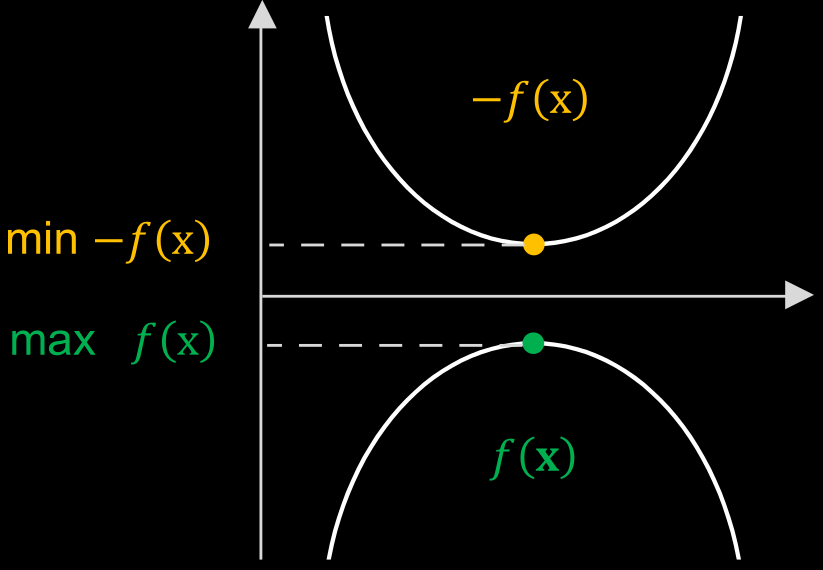
\includegraphics[scale=0.3]{Immagini/Screenshot From 2026-09-28 21-19-09.png}
            \end{center}
        \end{minipage}

        \section{Ottimizzazione}

            \subsection{Ottimizzazione non vincolata}
            La ricerca del/i punto/i di ottimo della funzione obiettivo viene condotta su tutto lo spazio di definizione della/e variabile/i di decisione

            \begin{center}
                \begin{minipage}{0.005\textwidth}
                    \begin{center}
                        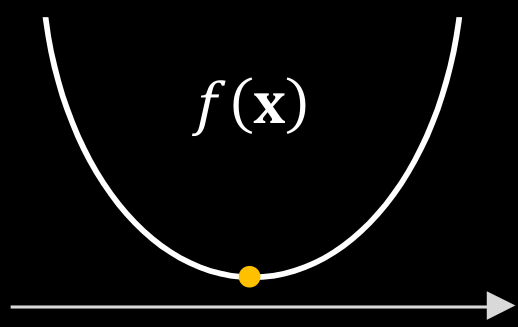
\includegraphics[scale=0.3]{Immagini/Screenshot From 2026-09-28 21-23-17.png}
                    \end{center}
                \end{minipage}
                \hfil
                \begin{minipage}{0.05\textwidth}
                    \begin{gather*}
                        X = \mathbb{R}^n \\ \\
                        x \in (-\infty, +\infty)
                    \end{gather*}
                \end{minipage}
            \end{center}


            \subsection{Ottimizzazione vincolata}
            La ricerca del/i punto/i di ottimo della funzione obiettivo viene condotta su un sottoinsieme proprio dello spazio di definizione della/e variabile/i di decisione

            \begin{center}
                \begin{minipage}{0.005\textwidth}
                    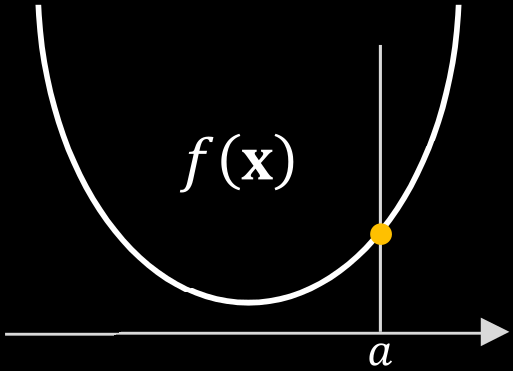
\includegraphics[scale=0.3]{Immagini/Screenshot From 2026-09-28 21-28-37.png}
                \end{minipage}
                \hfil
                \begin{minipage}{0.05\textwidth}
                    \begin{gather*}
                        X \subset \mathbb{R}^n \\ \\
                        x \in [a,+\infty)
                    \end{gather*}
                \end{minipage}
            \end{center}


            \newpage
            \subsection{Ottimizzazione Intera}
            Le variabili assumono solo valori interi

            {
                \large

                $$
                X \in \mathbb{Z}^n
                $$
            }

            \subsection{Ottimizzazione Binaria}
            Le variabili assumono solo valore 0 o 1

            {
                \large

                $$
                x \in \{0,1\}^n
                $$
            }

            \subsection{Ottimizzazione Mista}
            Alcune variabili assumono valori interi mentre altri variabili assumono solo valori binari

            Se non specificato altrimenti, si intende $X \subseteq \mathbb{R}^n$

    \newpage
    \section{Programmazione Matematica}
        \subsection{Definizione}
        Quando l'insieme $X$ delle soluzioni ammissibili di un problema di ottimizzazione viene espresso attraverso un sistema di equazioni e disequazione, esso prende il nome di \textbf{problema di programmazione matematica (PM)}

        \subsection{Vincoli}
        Un vincolo è un espressione del tipo,
        $g_i: X \to \mathbb{R} \quad
        g_i(\mathbf{x}) 
            \begin{Bmatrix} 
                \ge \\ = \\ \le 
            \end{Bmatrix} 0
        $ 
        è una funzione generica che lega tra loro le variabili decisionali, In generale possiamo avere uno o più vincoli.

        L'espressione $\begin{Bmatrix} \ge \\ = \\ \le \end{Bmatrix}0$ intende specificare che:
        \begin{itemize}
            \item $g_i(x) \geq 0$ oppure
            \item $g_i(x) = 0$ oppure
            \item $g_i(x) \leq 0$
        \end{itemize}

        \subsection{Definizione: Regione Ammissibile}
        In questo caso la regione ammissibile è definita dall'insieme dei vincoli del problema

        {
            \large

            $$
                X = \{x \in \mathbb{R}^n \text{ con } 
                g_i(\mathbf{x}) 
                \begin{Bmatrix} 
                    \ge \\ = \\ \le 
                \end{Bmatrix} 0, i=1,\dots,m
                    \}
            $$
        }
        
        Osserviamo, quindi, che abbiamo $m$ vincoli ed $n$ variabili
        \begin{itemize}
            \item Se $\mathbf{x \in X}$ allora $x$ è \textbf{soluzione ammissibile}
            \item Se $\mathbf{x \not\in X}$ allora x \textbf{non è una soluzione ammissibile (soluzione inammissibile)}
        \end{itemize}

        \subsection{Ottimi globali e locali}
        La risoluzione di un problema di programmazione matematica \uline{consiste nel trovare una soluzione ammissibile che sia un \textbf{otttimo globale}}, vale a dire un vettore $x' \in X$ tale che:
        
        \begin{gather*}
            f(x*) \leq f(x) \quad \forall x \in X \quad \text{se opt = min} \\ \\
            f(x*) \geq f(x) \quad \forall x \in X \quad \text{se opt = max}
        \end{gather*}

        Un problema di ottimizzazione può avere:
        \begin{itemize}
            \item Più di un ottimo globale
            \item Più di un ottimo locale
        \end{itemize}

        \subsection{Ottimi globali e locali: Casi possibili}

        \subsubsection{Programmazione lineare}
        {
            \large

            $$
                opt\, f(x) = c^Tx\, \text{(lineare)} \quad X = \{x \in \mathbb{R}^n :  
                g_i(\mathbf{x}) 
                \begin{Bmatrix} 
                    \ge \\ = \\ \le 
                \end{Bmatrix} 0, i=1,\dots,m
                    \}
            $$
        }

        \subsubsection{Programmazione lineare Intera}
        {
            \large

            $$
                opt\, f(x) = c^Tx\, \text{(lineare)} \quad X = \{x \in \mathbb{Z}^n :  
                g_i(\mathbf{x}) 
                \begin{Bmatrix} 
                    \ge \\ = \\ \le 
                \end{Bmatrix} 0, i=1,\dots,m
                    \}
            $$
        }

        \subsubsection{Programmazione non lineare}
        {
            \large

            $$
                opt\, f(x)\, \text{(lineare) o non lineare} \quad X = \{x \in \mathbb{R}^n :  
                g_i(\mathbf{x}) 
                \begin{Bmatrix} 
                    \ge \\ = \\ \le 
                \end{Bmatrix} 0, i=1,\dots,m
                    \}
            $$
        }

        \subsection{Esempio 1}

        \subsection{Esempio 2}

        \subsection{Esempio 3}

        \subsection{Esempio Cuba Libre}

        
    
    \part{Esercizi}

    \part{Laboratori}

\end{document}